%!TEX root = ../main.tex
\chapter{Appendix}
\label{ch:appendix}

This appendix collects supplementary material referenced throughout the
main text: (i)~confusion matrices at SNR $= 18$\,dB before and after
Adaptive-$K$ defense on the three optimization-based attacks, and
(ii)~representative per-SNR calibration values for the five classical
filter baselines used in Chapter~\ref{ch:evaluation}. All figures and
tables here support numbers reported in Chapter~\ref{ch:evaluation};
they are placed in the appendix to keep the main text focused on the
principal comparisons.

\section{Confusion Matrices under Optimization Attacks (SNR $= 18$\,dB)}
\label{app:confmat}

Figure~\ref{fig:confmat} shows the per-class confusion structure after
Adaptive-$K$ recovery for CW, EAD-L1, and EAD-EN at SNR $= 18$\,dB.
Across all three attacks, the recovered predictions concentrate on the
diagonal for the eight digital modulations, with residual confusion
localized to acoustically similar classes (QAM16 $\leftrightarrow$
QAM64) rather than distributed across all 11 classes as in the
undefended case. AM-SSB is preserved by the spectral-flatness routing
path (Chapter~\ref{ch:method}), which explains its consistent diagonal
recovery.

\begin{figure}[!ht]
  \centering
  \begin{subfigure}[b]{0.31\textwidth}
    \centering
    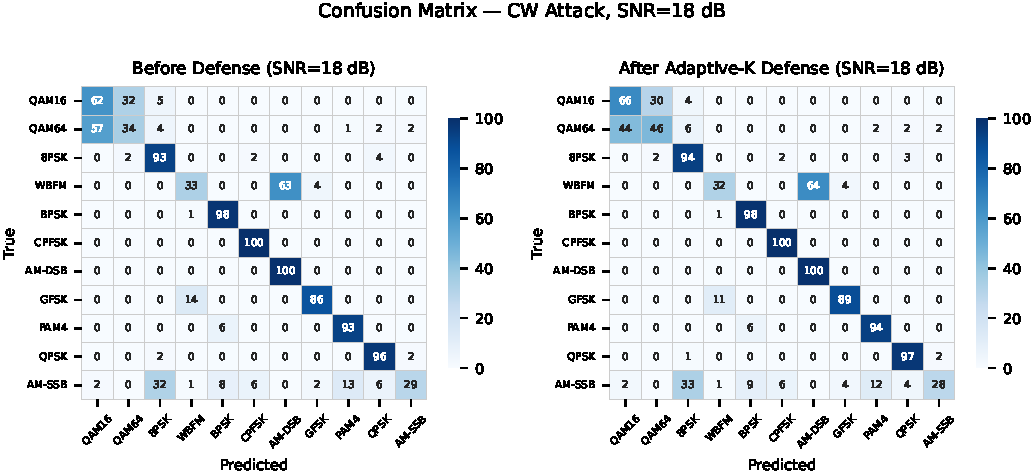
\includegraphics[width=\textwidth]{img/confmat_cw_snr18.pdf}
    \caption{CW (Adaptive-$K$).}
    \label{fig:confmat_cw}
  \end{subfigure}\hfill
  \begin{subfigure}[b]{0.31\textwidth}
    \centering
    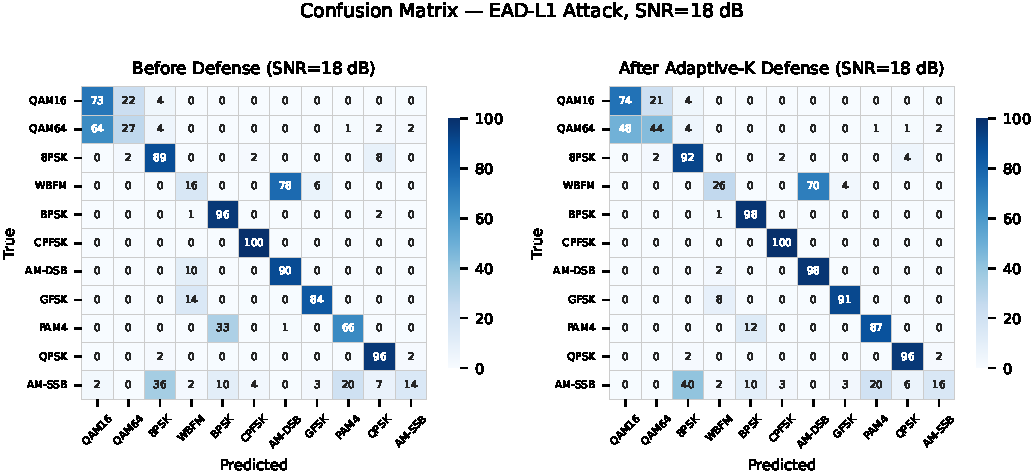
\includegraphics[width=\textwidth]{img/confmat_eadl1_snr18.pdf}
    \caption{EAD-L1 (Adaptive-$K$).}
    \label{fig:confmat_eadl1}
  \end{subfigure}\hfill
  \begin{subfigure}[b]{0.31\textwidth}
    \centering
    
\includegraphics[width=\textwidth]{img/confmat_eaden_snr18.pdf}
    \caption{EAD-EN (Adaptive-$K$).}
    \label{fig:confmat_eaden}
  \end{subfigure}
  \caption{Confusion matrices after Adaptive-$K$ recovery at
    SNR $= 18$\,dB. Residual off-diagonal mass is dominated by
    QAM16/QAM64 confusion (constellations that are hard to separate
    at any SNR), not by classifier collapse.}
  \label{fig:confmat}
\end{figure}

\section{Classical-Filter Calibration}
\label{app:calibration}

Table~\ref{tab:calibration} lists the per-SNR-calibrated hyperparameters
selected on the CW-adversarial validation set for the five classical
filters, at three representative SNR levels ($0$, $10$, $18$\,dB). These
values were obtained by grid search maximizing post-filter classification
accuracy on the undefended AWN model. The full calibration file
(\texttt{calibration\_params.json}) is loaded at test time; the settings
below are extracted from that file for illustration.

\begin{table}[!ht]
\caption{Representative per-SNR calibrated hyperparameters for the
  classical filter baselines. Values are the best-scoring configuration
  from the CW-adversarial validation grid search; the same
  configuration is applied to all attacks at test time, consistent
  with a deployment scenario in which the attack type is unknown.}
\label{tab:calibration}
\centering
\small
\begin{tabular}{llccc}
\toprule
Filter & Parameter & $0$\,dB & $10$\,dB & $18$\,dB \\
\midrule
Kalman         & $Q$              & 0.010 & 0.005 & 0.003 \\
               & $R$              & 0.010 & 0.001 & 0.001 \\
Wiener         & noise floor      & 0.020 & 0.010 & 0.005 \\
               & filter length    & 5     & 3     & 3     \\
Savitzky-Golay & window $w$       & 7     & 5     & 5     \\
               & polynomial deg.\ & 2     & 1     & 1     \\
Gaussian       & $\sigma$         & 0.8   & 0.5   & 0.3   \\
FIR            & cutoff $f_c$     & 0.10  & 0.15  & 0.20  \\
               & taps $M$         & 63    & 63    & 63    \\
\bottomrule
\end{tabular}
\end{table}

\section{Attack-Generation Latency}
\label{app:attack_latency}

Figure~\ref{fig:attack_bench} reports the per-batch generation latency
of the five evaluated attacks on our hardware. Optimization-based
attacks (CW, EAD-L1, EAD-EN) are one to two orders of magnitude slower
than gradient attacks (FGSM, PGD), reflecting the number of inner
optimization steps. Adaptive-$K$ defense latency (Table~\ref{tab:latency})
is comparable to a single FGSM invocation and negligible compared to
CW/EAD, supporting its use as an always-on receiver-side preprocessor.

\begin{figure}[!ht]
  \centering
  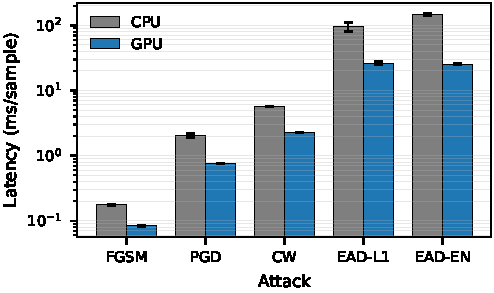
\includegraphics[width=0.7\textwidth]{img/attack_bench_latency.pdf}
  \caption{Attack-generation latency per batch of 64 samples for the
    five evaluated attacks. CW and EAD are dominated by their inner
    optimization loops (100 steps each); FGSM and PGD require only a
    small number of gradient evaluations.}
  \label{fig:attack_bench}
\end{figure}
